% 三棱柱拓扑示意；投影不按比例，虚线表示遮挡的棱/辅助连线。
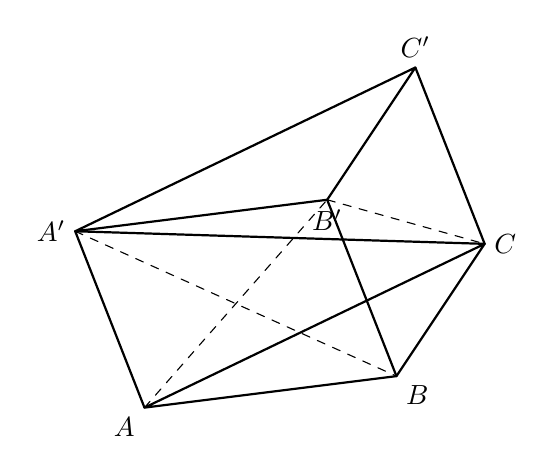
\begin{tikzpicture}[x=0.8cm,y=0.8cm,line cap=round,line join=round]
  \coordinate (A)  at (0,0);
  \coordinate (B)  at (4,0.5);
  \coordinate (C)  at (5.4,2.6);
  \coordinate (Ap) at (-1.1,2.8);
  \coordinate (Bp) at (2.9,3.3);
  \coordinate (Cp) at (4.3,5.4);
  \draw[thick] (A)--(B)--(C)--cycle;
  \draw[thick] (Ap)--(Bp)--(Cp)--cycle;
  \draw[thick] (A)--(Ap) (B)--(Bp) (C)--(Cp);
  \draw[thick] (Ap)--(C);
  \draw[dashed] (Ap)--(B) (A)--(Bp) (Bp)--(C);
  \node[below left] at (A) {$A$};
  \node[below right] at (B) {$B$};
  \node[right] at (C) {$C$};
  \node[left] at (Ap) {$A'$};
  \node[below] at (Bp) {$B'$};
  \node[above] at (Cp) {$C'$};
\end{tikzpicture}
